\documentclass{article}
\usepackage{amsmath}
\usepackage{tikz}
\usetikzlibrary{automata, positioning, arrows.meta}
\begin{document}
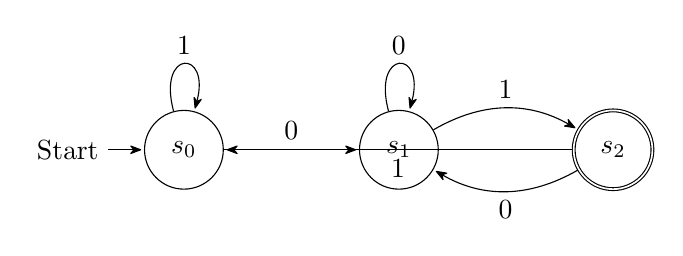
\begin{tikzpicture}[>={Stealth[round]}, shorten >=1pt, auto, node distance=2.5cm, every state/.style={minimum size=1cm}]
  \node[state, initial, initial text=Start] (q0) at (0, 0) {$s_{0}$};
  \node[state] (q1) at (2.73, 0) {$s_{1}$};
  \node[state, accepting] (q2) at (5.45, 0) {$s_{2}$};
  \path[->]
    (q0) edge node[auto] {$0$} (q1)
    (q0) edge[loop above] node[auto] {$1$} (q0)
    (q1) edge[loop above] node[auto] {$0$} (q1)
    (q1) edge[bend left] node[auto] {$1$} (q2)
    (q2) edge[bend left] node[auto] {$0$} (q1)
    (q2) edge node[auto] {$1$} (q0)
  ;
\end{tikzpicture}

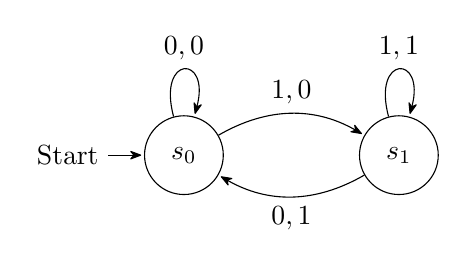
\begin{tikzpicture}[>={Stealth[round]}, shorten >=1pt, auto, node distance=2.5cm, every state/.style={minimum size=1cm}]
  \node[state, initial, initial text=Start] (q0) at (0, 0) {$s_{0}$};
  \node[state] (q1) at (2.73, 0) {$s_{1}$};
  \path[->]
    (q0) edge[loop above] node[auto] {$0, 0$} (q0)
    (q0) edge[bend left] node[auto] {$1, 0$} (q1)
    (q1) edge[bend left] node[auto] {$0, 1$} (q0)
    (q1) edge[loop above] node[auto] {$1, 1$} (q1)
  ;
\end{tikzpicture}

% \to marks the initial state s_0.
\begin{tabular}{c|cc|cc}
 & \multicolumn{2}{c|}{$f$} & \multicolumn{2}{c}{$g$} \\
State & $0$ & $1$ & $0$ & $1$ \\ \hline
$\to s_{0}$ & $s_{0}$ & $s_{1}$ & $0$ & $0$ \\
$s_{1}$ & $s_{0}$ & $s_{1}$ & $1$ & $1$ \\
\end{tabular}

% \to marks the initial state s_0; ^\star marks the final states F.
\begin{tabular}{c|cc}
 & \multicolumn{2}{c}{$f$} \\
State & $0$ & $1$ \\ \hline
$\to s_{0}$ & $\{s_{0}\}$ & $\{s_{0}, s_{1}\}$ \\
$s_{1}^{\star}$ & $\emptyset$ & $\emptyset$ \\
\end{tabular}

\[
M = (S, I, f, s_0, F)
\]
where
\[
\begin{aligned}
  &S = \{s_{0}, s_{1}, s_{2}\} \\
  &I = \{0, 1\} \\
  &f : S \times I \to S \\
  &F = \{s_{2}\}
\end{aligned}
\]

\[
G = (V, T, S, P)
\]
where
\[
\begin{aligned}
  V &= \{S, A, {\langle\text{noun}\rangle}, 0, 1, a\} \\
  T &= \{0, 1, a\} \\
  P &= \{S \to 0S1,\ S \to \lambda,\ A \to {\langle\text{noun}\rangle}a\}
\end{aligned}
\]
\end{document}
